\documentclass[
		a4paper,     % Format A4       
        twoside,     % zweiseitig %TODO undo
        BCOR=10mm,    % binding correction
        cleardoublepage=empty, % empties cleardoublepage=empty    
        parskip,     % Abstand zwischen Abs‰tzen, statt Einr¸ckung
        headsepline,  % separate heading and text by a line
        titlepage,   % mit Titelseite
        bibliography=totoc,    % include bibliography in TOC
%				liststotoc,
%       draft,       % renders faster, shows overfull boxes, doesn't render images
]{scrartcl}

% packages
\usepackage[ngerman, english]{babel} % choose your language with \selectlanguage{}
\usepackage[T1]{fontenc}
\usepackage[utf8]{inputenc} % ansinew avoids escaping german umlauts

\usepackage{verbatim}
\usepackage{graphicx} % graphics can be included using \includegraphics{}
\usepackage{textcomp}
\usepackage{amsmath,amssymb}
\usepackage{hyperref}
\usepackage{xcolor}
\usepackage{listings}
\usepackage[l3]{csvsimple}
\usepackage{caption}
\usepackage{subfigure}



% additional settings
\hypersetup{
 	pdfauthor={Frederic Rupprecht},
 	pdftitle={},
 	pdfsubject={Bachelor Thesis},
 	pdfkeywords={}
 	colorlinks=true,        % false: boxed links; true: colored links
 	linkcolor=black,        % color of internal links
	citecolor=black,        % color of links to bibliography
	filecolor=black,        % color of file links
	urlcolor=black          % color of external links
}
% style settings for json code
\colorlet{punct}{red!60!black}
\definecolor{background}{HTML}{e7e8ea}
\definecolor{delim}{RGB}{20,105,176}
\definecolor{json-key}{HTML}{29563a}
\lstdefinelanguage{json}{
    basicstyle=\small\ttfamily,
    % numbers=left,
    % numberstyle=\scriptsize,
    % stepnumber=1,
    % numbersep=8pt,
    showstringspaces=false,
    breaklines=true,
    frame=single,
    backgroundcolor=\color{background},
    morekeywords={role,content},
    keywordstyle=\color{json-key},
    literate=
      {":}{{"{\color{punct}{:}}}}{2}
      {",}{{"{\color{punct}{,}}}}{2}
      {\},}{{\}{\color{punct}{,}}}}{2}
      {\{}{{{\color{delim}{\{}}}}{1}
      {\}}{{{\color{delim}{\}}}}}{1}
      {[}{{{\color{delim}{[}}}}{1}
      {]}{{{\color{delim}{]}}}}{1},
}

% stretch text vertically by factor (zeilenabstand)
\renewcommand{\baselinestretch}{1.150}\normalsize

% avoid single lines at beginning/end of page
\clubpenalty10000
\widowpenalty10000

% custom hyphenation
\hyphenation{
% Ma-na-ge-ment  Netz-werk-ele-men-ten
% Netz-werk Netz-werk-re-ser-vie-rung
	BPMN---Community
}

\addtokomafont{sectioning}{\rmfamily}

% set path to image directory
\graphicspath{{images/}}

\lstset{
   basicstyle=\small,
   tabsize=4,
   showspaces=false, 
   showstringspaces=false, 
}

\tolerance=6000
\setlength{\emergencystretch}{3.0em}
\parskip8pt

\renewcommand{\descriptionlabel}[1]{
\normalfont\bfseries #1:}

\def\sectionautorefname{Kapitel}
\def\subsectionautorefname{Abschnitt}
\def\subsubsectionautorefname{Abschnitt}
\def\figureautorefname{Abbildung}
\def\lstlistingautorefname{Listing}


% my new commands
\newcommand{\quotes}[1]{``#1''}
\newcommand{\aref}[1]{\hyperref[#1]{A~\ref*{#1}}}


\begin{document}
	\selectlanguage{english}

	% special pages	
	\begin{titlepage}
	\begin{flushright}
		
\includegraphics[scale=.3]{hpi_logo_kl.jpg}
	\end{flushright}
	\begin{center}
		\hbox{}
		\vfill
		{\huge\bfseries Fine-Tuning Strategien zum Extrahieren von Event Logs aus Patienten Berichten \par}
		\vskip 0.5cm
		{\huge\bfseries Fine-Tuning Strategies for Extracting Event Logs from Patient Journeys \par}
		\vskip 1.5cm
		\textbf{Frederic Rupprecht}\\
		\vskip 1.5cm
		\begin{tabular}{l}
			Prof.~Dr.~Mathias~Weske \\
			MSc.~Jonas~Crimerius \\
		\end{tabular}
		\vskip 0.25cm
		\begin{tabular}{l}
			Lehrstuhl für Business Process Technology
		\end{tabular}
		\vskip 1.5cm
		\begin{tabular}{ll}
			Datum der Abgabe: & 30. Juni 2024 \\
		\end{tabular}
	\end{center}	
	\vfill
\end{titlepage}


	\cleardoublepage
	\thispagestyle{empty}
\vspace*{24\baselineskip}
\hbox to \textwidth{\hrulefill}
\par
Ich erkläre hiermit, dass ich die vorliegende Bachelorarbeit selbständig verfasst und keine anderen als die angegebenen Quellen und Hilfsmittel verwendet habe.

Potsdam, 01. Juli 2013
\newline
\newline
\newline
\newline
\newline
Name

\clearpage
	\cleardoublepage
	\thispagestyle{empty}
\vspace*{24\baselineskip}
\hbox to \textwidth{\hrulefill}
\par
I hereby affirm that I have written this bachelor's thesis independently, without using any sources other than those stated.

Potsdam, 01st Juli 2013
\newline
\newline
\newline
\newline
\newline
Name

\clearpage
	\begin{abstract}
Extracting event logs from natural language text is a discipline that gets more and more attention in academic circles, particularly with the advancement of large language models (LLMs) in the past years. On top of the challenges that exist when applying process mining on event logs extracted from traditional sources, additional hindrances arise with event logs based on natural language text. In order to address the challenges that the lack of structure and significant variance in natural language text pose in the extraction of information, fine-tuning LLMs for specific domains was researched in various fields of study. This thesis presents different approaches to fine-tuning a pre-trained model for extracting event logs from Patient Journeys. We thereby document the efficacy of established strategies for this use case. We focus on curating optimal training data sets and include details on the training process. Specifically, we apply supervised fine-tuning on GPT-3.5 Turbo with multi-task and single-task fine-tuning approaches. Our findings demonstrate promise, especially with multi-task fine-tuning, where the efficacy of fine-tuning is particularly pronounced. By evaluating the extraction on five metrics across four tasks, we present the fine-tuned model as superior in three of the evaluated tasks.
This research underscores the potential of fine-tuning LLMs to improve event log extraction from unstructured text, thereby enhancing process mining outcomes.
\end{abstract}
\clearpage
\begin{abstract}
Ereignissprotokolle aus natürlichsprachigem Text zu extrahieren ist eine Herausforderung, die in akademischen Kreisen im Laufe der letzen Jahre zunehmend Aufmerksamkeit bekommt, insbesondere durch die Weiterentwicklung von large langueage models (LLMs). Zusätzlich zu den Herausforderungen die beim Anwenden von Process Mining Techniken auf Ereignisprotokolle aus traditionellen Quellen entstehen, gibt es noch weitere Hindernisse wenn natürlichsprachlicher Text als Quelle verwendet wird. Fine-Tuning wurde bereits in einigen Forschungsbereichen eingesetzt, um die Probleme anzugehen die durch die mangelnde Struktur und die signifikante Varianz von natürlichsprachigem Text entstehen. Diese Arbeit zeigt verschiedene Ansätze, um ein vortrainiertes Modell für die Aufgabe Ereignisprotokolle aus Patient Journeys zu extrahieren, zu fine-tunen. Wir dokumentieren dabei die Wirksamkeit etablierter Strategien für diesen Anwendungsfall. Den Fokus legen wir dabei auf die Zusammenstellung optimaler Trainingsdaten und gehen detailliert auf den Trainingsprozess ein. Konkret wenden wir Supervised Fine-Tuning auf GPT-3.5 Turbo an und verwenden dabei multi-task und single-task Ansätze an. Unsere Ergbnisse sind vielversprechend, insbesondere unter Verwendung des multi-task Ansatzes. Durch Evaluierung von vier Schritten der Extraktion mit Hilfe von fünf Metriken zeigen wir die Überlegenheit des fine-tuned Modells in drei der vier Aufgaben.
Diese Arbeit verdeutlicht das Potenzial von Fine-Tuning, um die Extraktion von Ereignisprotokollen aus unstrukturiertem Text zu optimieren und dadurch die Qualität von Process Minings zu steigern.
\end{abstract}
	\cleardoublepage
	
	% listings
	\pagenumbering{Roman}
	\tableofcontents
	% \listoffigures
    % \lstlistoflistings
	\cleardoublepage
	
	% include your chapters
	\pagenumbering{arabic} 

	\section{Introduction}\label{sec:intro}
Over recent years, Process Mining has proven to be a powerful tool for detecting, analysing, and optimising (business) processes~\cite{weske_business_2012}. Its operation is fundamentally reliant on event logs, which traditionally are generated automatically within Information Systems.\\
However, with the rise of large language models (LLMs), interest in processing unstructured data has increased considerably. It would open up entirely new possibilities if we could analyse not only structured data from companies and healthcare systems, for example, but also non-standard reports from arbitrary individuals. These could range from analysing conversations from social media platforms such as Reddit or Facebook to specifically requested reports that do not adhere to a strict format, making them easier for people to produce.\\
Consequently, there is a crucial need to convert unstructured data into event logs, which is necessary to apply process mining. For instance, mamahealth is working on a project that utilises natural language testimonials from individuals with chronic illnesses. The project views these accounts from a process perspective, aiming to generate potentially life-altering insights.\\
The project TracEX, developed in collaboration with mamahealth, plays an essential role in this research and will be further introduced in the following chapters. It provides an extraction framework that this thesis aims to improve by providing fine-tuned models. There are significant challenges in sourcing and preparing data for Process Mining, even when using traditional data sources~\cite{van_der_aalst_process_2016}. From a practical standpoint, data quality is paramount for successful Process Mining. Any missing or untrustworthy event data severely undermines the value of the results obtained. 
\begin{quote}
    \quotes{From a practical point of view data quality is of the utmost importance for the success of process mining. If event data is missing or cannot be trusted, then the results of process mining are less valuable.}~\cite{van_der_aalst_process_2016}    
\end{quote}
These problems persist when using unstructured text as a data source. Furthermore, the data has to be structured, complicating matters even more. Non-standardised, non-automated data, written by laypeople without any claim for completeness or readability, are even more prone to the issues faced with traditional data sources.\\
In the past, attempts have been made to process this type of data, including in the realm of process modelling~\cite{friedrich_process_2011}. Aside from human manual extraction,  deterministic Natural Language Processing (NLP) approaches have been used. Unfortunately, these attempts quickly met limitations, particularly in deriving temporal relationships between events.\\
Recently, there has been an explosive rise in the field of Generative AI and LLMs in general. Transformer models from OpenAI, for instance, have proven to be powerful tools in various applications due to their ability to comprehend human language and respond in kind. This fact suggests that these models could also process textual disease course descriptions (patient journeys).\\
However, the use of LLMs introduces additional challenges. They are non-deterministic, meaning the same input can yield different outputs. Furthermore, their operation mechanisms are not transparent and, therefore, not entirely understood. Making them carry out tasks exactly as desired requires significant trial and error. For event logs, the quality and formatting of the collected data are vital. The data must not only be extracted accurately and completely but also cast into the appropriate format (such as XES).
These and many other hurdles pose substantial difficulties in event log extraction, as described in~\cite{munoz-gama_process_2022}. Established Transformer models, such as those from OpenAI, struggle to overcome these issues. Therefore, research has been conducted to explore ways to fine-tune these general-purpose models for specific tasks or topics. This work investigates the extent to which fine-tuning could solve these problems and create high-quality event logs. As stated by~\cite{latif_fine-tuning_2024}, 
\begin{quote}
\quotes{Fine-tuned GPT models are more suited to tasks like text completion, response evaluation, or open-ended queries because of their autoregressive nature, which excels in sequence formation.} 
\end{quote}

This thesis is structured as follows:\\
Chapter~\ref{sec:back} introduces t
he preliminaries followed by Chapter~\ref{related_work}, situating this thesis among other studies. Chapter~\ref{sec:fine} explores different approaches to fine-tuning and describes the compilation of training data. In Chapter~\ref{sec:eval}, the performance of the trained models is evaluated after introducing the required metrics. The thesis concludes with Chapter~\ref{sec:conclusion}, summarising findings, discussing the limitations and providing an outlook for future work.
    
\section{Preliminaries}\label{sec:back}
In this chapter, we introduce the terms and concepts used throughout the rest of the thesis. Where applicable, we use terms whose definitions are already established. At some points, we make minor adjustments to reduce complexity.\\\\ 
The success of the approaches we present later in this thesis is evaluated by evaluating event logs. So this is the first term we introduce.
\subsubsection*{Event Logs and Events}\label{sec:event-log}
Our definitions are based on~\cite{van_der_aalst_process_2016}.
As the name suggests, event logs are collections of recorded events and their defining data related to an observed process. They can be used as input for process mining and, therefore, must adhere to a particular structure. Usually, they are represented as tables, where each row represents one event, and each column contains the values of the events' attributes. The bare minimum for these attributes is \emph{case ID}, \emph{activity} and a timestamp to define an order between events. Each instance of the process from which the events originate is labelled with an ID, the case ID. All events related to the same case are referred to as a \emph{trace}. An event log can contain one or multiple traces. Activity is a description of the event that occurred, also called an activity label. On top of the mandatory attributes, more process-specific attributes can be recorded in an event log.\\
An event consists of a case ID, an activity label, a start timestamp, an end timestamp, an event type, and optionally other attributes such as the location where the event occurred. The activity label is a short description of the activity that took place. In the context of this thesis, it is not bound to a list of predefined terms or phrases. This means multiple activity labels can be syntactically different but semantically identical. An event is uniquely identifiable by the combination of its attributes. If the activity label of two events is semantically very similar while also sharing the same start timestamp, these two events are indeed the same event.\\\\
The source we want to extract events from is Patient Journeys. Since this term has no widely accepted definition, we clarify below how we use it in this thesis.

\subsubsection*{Patient Journeys}\label{sec:pj}
Patient Journeys are natural language texts without any defined format or structure. However, there are properties that are typically found in Patient Journeys: They describe a person's course of disease from the patient's perspective, as the patient themself usually writes it. It is agreed that the interaction between the patient and the health services, together with the following activities and interventions, are the critical components of a Patient Journey~\cite{ferrara_engaging_2019, kuo_rosacea_2015}. Characteristically, they encompass events spanning beyond, e.g. a single hospital stay, offering a broader picture by compiling experiences from before the onset of the condition, during hospital visits, at home, during doctor's appointments, and so on. Often, these accounts are enriched with personal feelings, either explicitly stated or implicitly conveyed through the writing style. The lack of structure and guidelines on what content must be included comes with advantages and disadvantages. Unlike doctor letters or automatic reports from Health Information Systems, they are more likely to be honest and approachable representations of how a patient perceives the course of disease.
On the other hand, Patient Journeys can have spelling and grammar issues, be of any length, and use mostly non-scientific phrasing. This makes any two Patient Journeys difficult to compare. They are commonly found online, notably on social media platforms such as X, Facebook, and Reddit.\\\\
The most essential tool in the extraction process we apply to create event logs from Patient Journeys is a GPT model. Therefore, we introduce the model we use in the following.

\subsubsection*{GPT-3.5}\label{sec:gpt3.5}
GPT-3.5 is an advanced language model developed by OpenAI, part of the GPT-3 series of models known for their capabilities in natural language processing. GPT-3.5 is designed to generate human-like text based on the input it receives, facilitating a wide range of applications from automated content creation to complex problem-solving tasks. Building on the architecture of its predecessors, GPT-3.5 utilizes a transformer-based model characterized by its use of self-attention mechanisms to balance the importance of various words in an input sequence~\cite{latif_fine-tuning_2024}. 
% Within this framework, self-attention calculates attention scores for each word relative to others in a sequence, allowing the model to emphasize significant words during text generation. Multi-head attention further refines this capability by employing multiple attention heads to capture various types of relationships and dependencies. 
In academic and practical contexts, GPT-3.5 has been recognized for pushing the boundaries of what language models can achieve. Despite its advancements, ongoing research continues to address its limitations and explore ways to improve the model's robustness, fairness, and interpretability~\cite {brown_language_2020}. GPT-3.5 Turbo is an advanced version of GPT-3.5. We use it in this thesis due to its API availability and fitting balance between capabilities and affordability.\\\\
The focus of this thesis is fine-tuning. To provide common ground, we outline the fundamentals we need to discuss our work.

\subsubsection*{Fine-Tuning}\label{sec:fine-tuning-def}
Fine-tuning Large Language Models (LLMs) means customizing their operation to align with the specific demands of a domain or task~\cite{ovadia_fine-tuning_2024}. Predominantly, a pre-trained LLM, such as a ChatGPT model, forms the foundation for this process, which primarily entails continuous training or iterative updates to the model's knowledge base. The objective here is to optimize the model's ability to manage domain or task-specific requests, which could relate to either knowledge or response behaviour, including response format.\\
There are multiple fine-tuning methodologies to boost the potential of LLMs, including supervised fine-tuning~\cite{zhou_enhancing_2024}, unsupervised fine-tuning, and reinforcement learning methods~\cite{touvron_llama_2023}. \emph{Supervised Fine-Tuning} (SFT) employs labelled input-output pairs, which implies that each instance in the training dataset is equipped with the intended output that the algorithm should independently generate. \emph{Unsupervised fine-tuning} uses unlabelled datasets, meaning there is no ground truth element. The model processes the data without specific instructions. This implies that the model uses methods like clustering and anomaly detection to find structure or patterns in the data. In \emph{reinforcement learning}, a model strives to optimize its performance in a specific task. It is an iterative approach that includes multiple rounds of feedback and a reward that depends on the models' performance. Intending to find the strategy that yields the greatest overall reward, the model continuously adapts and improves~\cite{ovadia_fine-tuning_2024}.
Another dimension in which one can differentiate fine-tuning strategies is the number of tasks a model is fine-tuned for.\\
\emph{Multi-task fine-tuning} means training a model on multiple related tasks simultaneously – within one dataset. By leveraging the commonalities of the tasks, the model can learn and understand quicker, decreasing the number of examples it needs to increase its performance in all the tasks~\cite{pilault_conditionally_2020}.\\
\emph{Task-specific fine-tuning}, on the other hand, means training a model for only one well-defined, isolated task. This enables an even more refined understanding of the intricate details of one specific task. Especially with very complex tasks or those that require a deeper understanding of the domain, this method excels~\cite{xinxi_single_2021}.

\paragraph{Training Data}
When using SFT, the model learns solely from examples. In the context of OpenAI's models, the process functions as follows: The model is given a system message, a user message, and an assistant message. The system message describes the behaviour the model should adopt and the task it should perform. The user message contains the input on which the model should perform the task. The assistant message then contains the desired answer – the response the model should give when confronted with this task in the future.
One message set closely resembles one turn of a regular exchange with ChatGPT, with the difference being that the answer is also given to the model instead of the model calculating the answer itself. \autoref{lst:fine-tuning-example} shows an example for a message set.
\begin{lstlisting} [language=json, caption={Example for fine-tuning training data}, label={lst:fine-tuning-example}]   
{"messages":[
    {"role":"system",
     "content":"You are an expert in text categorization. Your job is to take a given activity label and to classify it into one of the following event types: 'Symptom Onset', 'Symptom Offset', 'Diagnosis', 'Doctor Visit', 'Treatment', 'Hospital Admission', 'Hospital Discharge', 'Medication', 'Lifestyle Change' and 'Feelings'. Please consider the capitalization."
    },
    {"role":"user", "content":"testing positive for Covid19"},
    {"role":"assistant","content":"Diagnosis"}]}
\end{lstlisting}
The training data is made up of ten to hundreds of examples.\\\\
We use an open-source project as a foundation for our work and as a reference to measure our accomplishments in this thesis. Because of that, we introduce the project's core functionalities and concepts.

\subsubsection*{TracEX}\label{sec:tracex}
TracEX is an LLM-based data processing pipeline that aims to extract event logs from Patient Journeys. It takes a Patient Journey as an input and delivers an event log as an output. The extraction process involves many steps, some of which are important in the context of this thesis. Hence, they are listed below:
\paragraph{Preprocessing} Patient Journeys are often unstructured, making it hard to extract information from them. Events are not always described in chronological order, time-related information is often missing or relative to each other (e.g. \quotes{two weeks later}), and language is not standardized (use of synonyms, paraphrases or slang). Extracting data from this reliably is virtually impossible. This is why preprocessing is essential. The Patient Journey is moulded into a more structured format in order to streamline the following steps while still retaining the continuous text format. This process includes correcting spelling and grammar as well as identifying and transforming time-related phrases into a date format (e.g. YYYY-MM-DD). Additionally, case information like the author's age and the described condition are extracted.
\paragraph{Labelling Activities} All relevant events are determined using the entire Patient Journey as context information and also considering the condition. They are then each summarized into six words at most. This implies that the exact phrasing of an activity label can vary each time the pipeline is executed. An example of a typical activity label is \quotes{experiencing fever-like symptoms}.
\paragraph{Extracting Event Types} Given an activity label, the category of that activity is determined from a predefined list. Possible event types are: Symptom Onset, Symptom Offset, Doctor Visit, Hospital Admission, Hospital Discharge, Treatment, Medication, Lifestyle Change and Feelings.
\paragraph{Extracting Timestamps} Given an activity label, its start and end date are determined. It is extracted if possible and extrapolated if not. Furthermore, the duration of the activity is calculated from the two timestamps.\\\\
To achieve the described outcome, a mix of deterministic scripts and requests to the OpenAI API are used. Among other techniques, prompt engineering is used to increase the quality of the extracted event logs.
The few-shot prompting technique has proven to be especially suited for the described tasks. A request to the OpenAI API might contain a message list like displayed in \autoref{lst:few-shot}, where \verb|activity_label| is the appended input that should be used in the extraction, while all previous user and assistant messages are few-shot examples.
\begin{lstlisting}[language=prompt, caption={Few-shot prompt to categorize activities into event types}, label={lst:few-shot}]
system: You are an expert in text categorization and your job is to take a given activity label and to classify it into one of the following event types: Symptom Onset, Symptom Offset, Diagnosis, Doctor Visit, Treatment, Hospital Admission, Hospital Discharge, Medication, Lifestyle Change and Feelings. Please consider the capitalization.  
user: visiting doctor's 
assistant: Doctor Visit  
user: tested positive for Covid19
assistant: Diagnosis
user: activity_label  
\end{lstlisting}
A prompt containing the task for the model and a list of examples to specify the models' behaviour is given, along with the activity label to be classified.
Please note that TracEX is an open-source tool. It may still be in development, and functionality might be altered, removed or added in the future. The development status this thesis builds upon can be checked in the repository\footnote{https://github.com/FR-SON/TracEX}.

	\section{Related Work}
\label{sec:related_work}
Using LLMs to extract event logs from natural language text (NLT) combines the complexity of several research disciplines: Natural Language Processing (NLP), Information Extraction (IE), Prompt Engineering, Modelling (wherein the configuration of event logs is a design decision), Software Engineering and LLM-training.\\
In this bachelor thesis, we focus explicitly on fine-tuning and the specific application of all these disciplines to extracting event logs from Patient Journeys. This use case has been relatively under-researched and is currently not documented.\\\\
In essence, extracting event logs from Patient Journeys is an IE task. IE tasks aim at extracting information from unstructured plain text. Han et al.~\cite{han_is_2023} conducted extensive research on how well ChatGPT performs in IE tasks. The outcome revealed that, even with the usage of all common prompt engineering approaches (e.g. Few, Shot, Chain of Thought), ChatGPT lags considerably behind State-of-the-Art methods. Outcomes are even worse – up to 48\% – when irrelevant information for the task is included in the context.\\
Bahak et al.~\cite{bahak_evaluating_2023} also emphasized that GPT-3.5 Turbo often hallucinates by giving context-related responses to questions, even though the given context does not contain an answer. This problem is also encountered when extracting from Patient Journeys due to often missing information, particularly time specifications. Hence, this study investigates whether fine-tuning can mitigate the problem.\\\\
Ovadia et al.~\cite{ovadia_fine-tuning_2024} explored various fine-tuning strategies (mainly unsupervised fine-tuning (USFT) and retrieval-augmented generation (RAG)) aiming to improve the processing of knowledge-based tasks. They discovered that knowledge-based tasks could be significantly improved using fine-tuned models, but RAG is more suitable for knowledge injection than USFT. Contrarily, our approach aims to enhance the model's output not by adding more knowledge but by helping the model better understand the complex task at hand. Therefore, our pursuit requires different demands on fine-tuning strategies.\\\\
\newpage
Latif et al.~\cite{latif_fine-tuning_2024} explored fine-tuned ChatGPT's potential in automated scoring of students' written work. They employed a large, diverse dataset to train their model. The result showed that the outcomes were not only better than those of the base model ChatGPT but also surpassed the performance of the then-best publicly available model, BERT. The tasks to be corrected were single and multi-label tasks, so primarily multiple-choice questions. This bachelor thesis mainly deals with tasks without predefined answer options. These tasks are even harder for the model to complete correctly and also require a different evaluation approach.\\\\
In other research areas such as Caption Rewrites~\cite{gladkoff_predictive_2023}, News Recommendations~\cite{li_exploring_2023}, or Machine Translation Evaluation~\cite{wang_mitigating_2023}, research confirmed that the application of fine-tuned models led to improved results.\\\\
A common thread in these studies is the utilization of large, well-established datasets. Extracting event logs from NLT, or Patient Journeys specifically, is still a niche sector in which such datasets do not exist. Hence, the compilation of these datasets, a crucial part of this Bachelor's Thesis, is conducted with utmost care and thoroughness to ensure the reliability of our findings.\\\\
In short, the GPT-3.5 Turbo base model is not very adept at performing IE tasks and suffers greatly from too large contexts. Depending on the goal, different fine-tuning strategies might be better suited to customize an LLM in the desired way. The increased performance of fine-tuned pre-trained transformer models in various fields of study is promising. However, the fact remains that extracting event logs from NLT involves problems that were not tackled before. The ambition of this bachelor thesis is to extend the aforementioned findings and determine if fine-tuning can resolve IE-task problems by applying training strategies. The objective of extracting high-quality event logs from Patient Journeys is used as an example throughout this thesis, as it is the focus of the underlying tool, TracEX.
    \section{Fine-Tuning Strategies}\label{sec:fine}
In the following chapters, we will present an approach to fine-tuning GPT-3.5 Turbo, that is specialized for the task of extracting event logs from Patient Journeys. We will use four of the steps used in TracEX to demonstrate: Extracting activity labels, classifying event types, extracting start timestamps and extracting end timestamps. Part of that approach is preparing the datasets for training and validating the model. This is mainly due to the fact, that the desired application is a niche subject which results in a lack of large, established datasets. Curating and assembling the training data is a time-consuming yet crucial task in fine-tuning an LLM.\\\\
Since we use GPT-3.5 Turbo and the corresponding tools from OpenAI, the set of applicable fine-tuning strategies is limited. As mentioned in \ref{sec:fine-tuning-def} there are fundamentally 3 different strategies, that are potentially interesting: Supervised fine-tuning (SFT), unsupervised fine-tuning and reinforcement learning. The fine-tuning framework OpenAI provides is focused on SFT, so that is what we focus on as well. Fittingly, SFT is said to be suited for improving a model's understanding of complex tasks and increasing the reliability of correctly formatted responses, which is the purpose we use fine-tuning for.\\
Another dimension in which one can differentiate fine-tuning strategies is the number of tasks a model is fine-tuned for.\\
\emph{Multi-task fine-tuning} means training a model on multiple related tasks at the same time – within one dataset. By leveraging the commonalities of the tasks, the model can learn and understand quicker, decreasing the number of examples it needs to increase its performance in all the tasks.~\cite{pilault_conditionally_2020}\\
\emph{Task-specific fine-tuning} on the other hand means training a model for only one well-defined, isolated task. This enables an even more refined understanding of the intricate details of one specific task. Especially with very complex tasks or those that require a deeper understanding of the domain, this method excels.~\cite{xinxi_single_2021}\\\\
The individual steps included in the extraction framework of TracEX can be categorized into different types of tasks. Each type poses different challenges and has a different complexity. The classification of event types requires the GPT to select the correct answer from a predefined set of choices. On top of that, the given context is relatively small. Determining the relevant activities is a much more complex task and the GPTs response is only limited by the number of words that should represent one activity. The exact words that make up the activity is up to the GPT to decide. The context for that task is larger as well, since all sentences have to be examined in context in order to determine which activities are relevant and which descriptions make up one event in the Patient Journey. Deriving timestamps for activities is without a doubt the hardest task. Not only is temporal information often hardly present or missing all together in real-world Patient Journeys, but can also take many shapes. 'On 2024/04/02', 'at the beginning of August', 'On Tuesday', 'In autumn', 'As the week progressed', 'Later' are all examples from real-world Patient Journeys, that need to be converted into XES-conform timestamps. So, adding to all the challenges involved in this type of task, is the requirement for correct formatting.

\subsection{Multi-task fine-tuning}\label{sec:multi-task-ft}
In this chapter, we will describe the process of multi-task fine-tuning GPT-3.5 Turbo for all the mentioned tasks – labelling activities, classifying event types,  determining start timestamps and determining end timestamps. This strategy counteracts the fact, that the size of the datasets will always be relatively small, compared to the datasets used in the work presented in ~\autoref{related_work}. Examples that explain the classification of event types for instance, take activity labels as input, which means this step also profits from the examples for extracting activity labels, because more possible activity labels are presented throughout the training process. The underlying task in all steps is to understand, extract and transform information from a text. This makes it a valuable approach.

\subsubsection{Curating Datasets}\label{sec:curating_data}
We structure this chapter into three paragraphs. Each paragraph describes one of the message types we need in our fine-tuning training data. tarting with system messages, then user messages and finally assistant messages. Furthermore, each paragraph sequentially describes the characteristics of the different messages for activity labelling, start and end timestamp extraction and event type classification.
\paragraph{System Messages:} The system message is in most cases identical to the system prompt used in TracEX – for two reasons:
\begin{enumerate}
    \item
        The prompts are complex, specifying the thought process the model should take, the format of the response and which aspects of the input to focus on. Showing the model how to respond to these specific instructions underlines the connection between the details of the instructions and the desired output. For example, if the instruction includes \quotes{Answer, using only one word.} and the assistant-message contains only one word, it should be easier for the model to understand how to action this instruction in the future. Thus, the training data prepares the model for the exact instructions it will be prompted with.\\
        The drawback of this approach is, that the prompts used with the fine-tuned model can not be shortened as much. They still need to contain every specification that is necessary for the base model. On the other hand, this makes the model more flexible: If a prompt contains special instructions, they will be implemented. If a prompt does not contain special instructions, no predefined formatting or similar customizations will pre present in the response.\\
        Teaching a model to behave in a certain way purely by examples – omitting the explanations in the system messages, but keeping the output the same – can also work. But because the fine-tuned model has no connections between the instructions and the demanded behaviour, it will always behave like the examples taught it to, making it less flexible. That is why we do not choose this approach.
    \item 
        Showing the model the exact same instruction over and over again, should result in the model being primed to fulfil that task, without being 'distracted' by other possible instructions. It knows only this one task, to exaggerate. Of course, a pre-trained model like GPT-3.5 Turbo has vast knowledge about various other tasks. Fine-tuning only changes the model on the surface level. Still, this should be considered, which is why we propose the approach of keeping the system prompts close to ones that will actually be used with the fine-tuned model.
\end{enumerate}
\autoref{lst:system:starttime} shows what a system message can look like.

\begin{lstlisting}[language=json, caption={System message for determining an activies start timestamp}, label={lst:system:starttime}]
{"role":"system",
 "content":"You are an expert in text understanding and your job is to take a given text and a given activity label and to extract a start date to this activity label. Only output the extracted start date! Rely on the context to determine the start date, as it might not be explicitly mentioned."
}
\end{lstlisting}

\paragraph{User messages:}\label{par:user-messages} Sample tasks in the user-messages should also be similar to the ones the fine-tuned model will face in reality. The training data contains example inputs like they are described in \autoref{sec:tracex}:\\
Training data for the activity labelling step is an entire patient journey. The goal is to convey which parts of the huge context are important. In order to demonstrate which aspects to keep and which to discard in the assistant-message, the entire journey is necessary.\\
To illustrate, assume a patient journey contains the following paragraph:
\begin{quote}
    \quotes{As soon as I regained my strength, I scheduled an appointment to receive the Covid-19 vaccine. I received the first dose of the vaccine and plan to get the second one after the recommended time between shots.}
\end{quote}
The GPT might extract  \quotes{regaining strength}, \quotes{scheduling appointment for vaccination} and \quotes{receiving first dose of Covid-19 vaccine} as the relevant events. Mentioning the appointment in the event log is superfluous, since the text states explicitly, that the vaccine was received and that is the relevant information. So, the correct answer should be \quotes{regaining strenght} and \quotes{receiving first dose of Covid-19 vaccine}, while the rest is omitted.\\
Without knowing, that the second sentence is part of the Patient Journey and without understanding the relation between the two sentences, the GPT can not give a correct answer. That is why providing a large context is important for this task.\\
To teach the model which events are relevant and which are not, we also include examples that contain a lot of irrelevant information the model should ignore. In the assistant messages, we can then omit the irrelevant information from the summaries.\\
In addition to complete Patient Journeys, short excerpts from Patient Journeys, are also viable examples. They fulfil a different purpose. Aside from understanding the situation described in the Patient Journey and isolating the relevant events, the model also needs to be trained on how to output its findings. Providing a multitude of shorter examples, creates a blueprint on how actives should be summarized. Active or passive writing style, rephrased or close to the original text, past or present tense are options that should be defined. More on that in the next paragraph.\\\\
Examples that train for the extraction of start timestamps contain an activity label, representing the event, and an excerpt of the original Patient Journey which the activity label was extracted from before. This is also the approach chosen in TracEX. The method delicately balances providing the GPT with sufficient context to understand the temporal relations of an event against limiting the volume of data. This ensures the performance of the GPT is not impaired due to an excess of irrelevant information for the given event~\cite{han_is_2023}.\\\\
Examples for end timestamps work similarly, additionally containing the previously extracted start timestamp. The start timestamp can be a great indication for the end timestamp of an event. Providing it makes it easier for the model to understand which event is the current one, thus ensuring start and end timestamp refer to the same event. Furthermore, more often than not, the end timestamp is not stated at all in the Patient Journey. With knowledge about the start timestamp, the GPT can make better estimations on when the event ended.\\
In this way, the fine-tuning examples are structured just like the messages, the model will be prompted with. Especially concerning timestamps, the input examples need to be diverse. By providing input with different variations of timestamps as described before allows us to later on provide the model with  correct responses to these varying timestamps. This way, the fine-tuned model is more likely to recognize relative specifications like \quotes{during that time} and handle them in a desirable way. \\
User messages for the training of classifying event types are the most straight forward. They consist of just one activity label, that should be classified.\\
\autoref{lst:user:starttime} shows what a user message could look like.
\begin{lstlisting}[language=json, caption={User message for determining an activities start timestamp}, label={lst:user:starttime}]
{"role":"user",
 "content":"I started experiencing flu-like symptoms in July 21. I then got tested positive for Covid19. In October I got infected again. Then on the 4th of November I got my first dosage of the vaccine. I had heavy side effects.\n Activity Label: starting to experience symptoms"
}
\end{lstlisting}

\paragraph{Assistant messages:} An assistant message for activity labelling consists of three to six word summaries of events from the respective Patient Journey. The approach we follow is to keep the summaries close to the original text, regarding the choice of words. As described in \autoref{sec:tracex}, the created activity label is later on also used to determine the event type and timestamps. To make it easier for the GPT to recognize the activity by its label in the original text, the words should be not too far off. For instance, in ~\autoref{lst:user:starttime} an activity label is used to indicate which of the timestamps present in the context is the relevant one for this request. If that activity had been summarized to \quotes{symtom onset} or \quotes{noticed first symptoms} the model might have a harder time matching activity and timestamp, because the event in question is not recognized.\\
That means the model does not learn to always use a certain structure for the summaries or a specific tense, but to adjust it to the given input instead. The focus of these examples is to provide guidance on which information is important and which is not. A user message that contains only one relevant event and spans 5 sentences is reduced to just one activity label, representing the one relevant event.\\\\
Assistant messages for classifying event types are just the event type itself, from the predefined list. Repeating this output format in every example of the training data teaches the model, that no accompanying text is allowed. Otherwise, GPT-5.5 Turbo tends to include phrases like \quotes{Certainly, here is the event type for your activity}. This makes using and also evaluating the results much harder, so training the model on the output format is very helpful. \\\\
A similar approach is applied for the time stamps. By defining a format for the timestamps and repeating it in every example, the output is formatted correctly a lot more reliably. The timestamp format required for XES files is \verb|YYYMMDDTHHMM|, so that is what we use.\\
\autoref{lst:assistant:starttime} shows what an assistant message could look like.
\begin{lstlisting}[language=json, caption={Assistant message for determining an acitivities start timestamp}, label={lst:assistant:starttime}]
{"role":"assistant","content":"20210701T0000"}
\end{lstlisting}

The messages shown in ~\autoref{lst:system:starttime}, \ref{lst:user:starttime} and \ref{lst:assistant:starttime} combine to one element in the training data.\\\\

Fine-tuning in our case requires training data that comprises both answerable and non-answerable examples. In particular, it is crucial to provide ample examples where the context supplies sufficient information for the model to deliver an answer, and just as important, examples where the context is insufficient, making it impossible for the model to provide an answer. The ultimate goal of this juxtaposition is to teach the model to effectively differentiate between contexts where an answer can be procured and where it can not.\\
For instance, a lack of specific data, like a timestamp, might result in 'N/A' being the most fitting answer the model can deduce. However, it has been found that GPT-3.5 Turbo often defaults to 'N/A' even when the required information is present. This necessitates that the training data meticulously demonstrates both instances where there genuinely is no answer, separated from situations where an answer should indeed be provided. This encourages the model to refrain from utilizing 'N/A' as a response unless it’s genuinely the only valid option left.\\
Furthermore, the training data should strike a balance between simple and complex cases. A sufficient amount of straightforward instances is necessary to cement a clear understanding of rudimentary functioning steps. At the same time, a generous presence of complicated examples is essential to equip the model with the necessary adaptability and problem-solving skills. As mentioned in \ref{par:user-messages} the context from which to extract activity labels can be a complete patient journey, thereby containing multiple examples for the mapping of sentences to activity labels.  This allows us to create simple and complex examples from just one Patient Journey. A set of one to four sentences makes a rather simple example. Three or four of these sets at once make a much harder, yet more realistic, task. The approach we implement is to first use the simple examples and follow up with one large example, combining the simpler ones. You can see a shortened example of that in~\autoref{lst:combined-example}.
\begin{lstlisting}[language=json, caption={Simple and complex examples for determining acitivity labels}, label={lst:combined-example}]
{"messages":[
    {"role":"system","content":..."},
    {"role":"user","content":"0: After experiencing the first symptoms of Covid-19 on 2020/09/13, I immediately isolated myself at home to prevent the possible spread of the virus to my family 1: My symptoms started with a mild fever, fatigue, and a dry cough, which progressively worsened over the following days"},
    {"role":"assistant","content":"First symptoms: Mild fever, fatigue, dry cough #0\nIsolated at home #0\nSymptoms worsened #1"}]}
{"messages":[
    {"role":"system","content":"..."},
    {"role":"user","content":"2: By 2020/09/15, I developed difficulty breathing and chest pain, prompting me to consult with a doctor via telemedicine 3: The doctor advised me to monitor my symptoms closely and prescribed medications to alleviate fever and cough."},
    {"role":"assistant","content":"Developed difficulty breathing, chest pain #2\nConsulted doctor via telemedicine #2\nDoctor prescribed medications #3"}]}
{"messages":[
    {"role":"system","content":"..."},
    {"role":"user","content":"0: After experiencing the first symptoms of Covid-19 on 2020/09/13, I immediately isolated myself at home to prevent the possible spread of the virus to my family 1: My symptoms started with a mild fever, fatigue, and a dry cough, which progressively worsened over the following days 2: By 2020/09/15, I developed difficulty breathing and chest pain, prompting me to consult with a doctor via telemedicine 3: The doctor advised me to monitor my symptoms closely and prescribed medications to alleviate fever and cough"},
    {"role":"assistant","content":"First symptoms: Mild fever, fatigue, dry cough #0\nIsolated at home #0\nSymptoms worsened #1\nDeveloped difficulty breathing, chest pain #2\nConsulted doctor via telemedicine #2\nDoctor prescribed medications #3"}]}
\end{lstlisting}

\subsubsection{Data Sources}\label{sec:data_sources}
This chapter outlines how we acquire and prepare the data we use to fine-tune the model.In the process of acquiring training data for fine-tuning, three main steps are employed:\\\\
Firstly, sample data that can serve as input is collected. This includes gathering real-world patient journeys and potentially making minor adjustments to ensure their utility as examples. We need to make sure that the training data features input that the base model struggles with in order to demonstrate how those cases should be handled by the fine-tuned model. Additionally, synthetic patient journeys are generated, because of their clear structure and completeness. Hence, they are well-suited for serving as basic training examples for the core aspects of extraction and also for validation.\\\\
Secondly, the TracEX pipeline is utilized to establish a starting point for extraction results. This process entails incorporating few-shot prompts from TracEX into the training data, as these are already excellent examples. The pipeline is then executed using the collected Patient Journeys and the intermediate results of the pipeline are logged in a suitable JSON format compatible with use as training data. Each step we intend to fine-tune the model for is represented in the intermediate results. For instance, the system and user message utilized in TracEX' query to the ChatGPT API is copied and the API's response is used as the assistant message. This way, each execution of the pipeline produces one set of messages, that can be used as training data. However, manual checking and corrections are absolutely necessary at this stage, as errors occur, thereby compromising the training examples. It is crucial that the training samples are free from fault, otherwise, this could propagate the faults into the fine-tuned model. Naturally, these intermediate results are mearly a starting point. If TracEX could already extract the required information so well it could be used as fine-tuning training data, fine-tuning would not be required at all.\\\\
Lastly, ChatGPT 4 is requested to do the same extraction tasks as TracEX and the results are used as examples in the training data as well. ChatGPT 4 outputs outperform those from GPT-3.5 Turbo and exemplify what the fine-tuned model should achieve after fine-tuning. Nonetheless, the results still need further human refining and adjustments. In order to curtail costs, the batch-upload feature from OpenAI is used to make many of the required requests to the API, as it is cheaper.

\subsubsection{Parameters}
OpenAI provides three key hyperparameters that allow for customization of the fine-tuning process~\footnote{\href{https://platform.openai.com/docs/api-reference/fine-tuning/create\#fine-tuning-create-hyperparameters}{OpenAI API documentation}}: epochs, batch size, and learning rate multiplier. Epoch refers to one complete pass through the entire training dataset. Increasing it makes the models answers comply more closely to the training data. This can also lead to overfitting, which is especially harmful for tasks that allow more varied answers. Since our set of tasks involves such tasks but also ones that require very specific answers, we opt to use two epochs. The batch size parameter determines the number of training examples used in one iteration to update the model’s parameters. Given our relatively small dataset of around 100 examples across four tasks, we choose a batch size of one to maximize the utility of each training example. It is worth noting, that these 100 examples amount to about 32000 tokens or 24000 words. The learning rate multiplier adjusts the base learning rate, which controls how much the model’s weights are updated with respect to the calculated error after each epoch. Due to the limited training data, we opted for a learning rate multiplier of 2 to enable the model to learn more quickly. 

\subsection{Single-task fine-tuning}\label{sec:single-task-ft}
In this chapter, we will describe the process of task-specific fine-tuning for one task. For this purpose, we choose to train a model for extracting activity labels from Patient Journeys. This task is one of the most difficult among the tasks we introduced so far and is also a more interesting subject than a traditional classification task, such as done in the event type classification step.\\
Extracting activity labels for events in Patient Journeys is a complex task. It requires an understanding of the condition at hand, because it also implies determining which of the mentioned activities are relevant for the case. Fine-tuning an LLM for a single task allows us to focus on more of the issues a model has with performing the task. By providing even more examples in the form of training data, we intend to teach the model how to handle difficult tasks, without diverging the attention of the model by introducing other tasks, like we did in \autoref{sec:multi-task-ft}. This makes it a valuable approach.\\\\
Curating datasets is and the data sources for this model are very similar to the process described in \autoref{sec:data_sources} and \autoref{sec:curating_data} respectively. All approaches described for collecting examples for the task of labelling activities applies to the training of the single-task fine-tuned model as well. The sole difference is, that \emph{all} examples we train the model with are specific to labelling activities.\\\\
The training data for this model contains 50 examples for the task "Activity Labelling". This is double the amount the multi-task fine-tuned model got. This amounts to approximately 16000 tokens. Because this set of training data is more specialized but still smaller overall we choose to adjust the Hyperparameters: 3 Epochs, Batch Size 1 and LR-Multiplier 2.

\subsection*{Summary}
The process of fine-tuning a GPT model for information extraction tasks starts with collecting or generating sample data from which to extract the information. Next, ground-truths for individual texts need to be created in order to create examples the model can learn from. The examples need to be manually validated and adjusted to ensure they are free from any faults, that would otherwise harm the model's performance. Depending on the kind of task-mix the model should later on perform and number of total examples in the training data and suitable hyperparameters need to be chosen. The training data needs to address the problems the base model has, by providing examples and possible answers, so the model can learn how to handle the problematic cases. High quality as well as high quantity of the training data is crucial.

    \section{Evaluation}\label{sec:eval}
In this chapter we will evaluate the presented approaches by using the trained models from Chapter~\ref{sec:multi-task-ft} and \ref{sec:single-task-ft} to extract event logs from patient journeys. In order to properly compare the fine-tuned models and the base model, we will first introduce the metrics we use. Second, we will describe the evaluation process. Third, we will present our results for each model, each task and each of the task's metrics individually.\\
The evaluation is based on comparing the extracted event logs to a ground truth and determining the differences between them. This is one out of a few options already established in the academic context~\cite{latif_fine-tuning_2024}.

\subsection{Metrics}\label{sec:metrics}
In \ref{sec:multi-task-ft} we describe the process of fine-tuning a model to perform multiple related tasks. We evaluate each of these tasks individually. The model trained in \ref{sec:single-task-ft} performs only the task \quotes{Activity Labeling}, so we use the metric described in \ref{sec:activity_metrics} as well.

\subsubsection{Activity Labelling Metrics}\label{sec:activity_metrics}
There already are established metrics in the process mining sector we can use to determine if an event log is of good quality in terms of activities.~\cite{van_der_aalst_process_2016, carmona_conformance_2018} They propose three categories an activity can have. We use similar categories for the activity labels.\\
It is worth noting, that determining if one activity label from the evaluated event log and one from the ground truth are indeed the same activity label is not as straight forward as one might think. As discussed in \ref{sec:tracex}, the activity labels are not predetermined, instead they are chosen by the model that extracts them. This means two activity labels can be syntactically different but still describe the same activity. For the purpose of this evaluation, we define two activity labels as identical, if they are semantically very similar.
\paragraph{Missing Activity} An activity is missing, if it is featured in the ground truth, but not in the evaluated event log. 
\paragraph{Unexpected Activity} An activity is unexpected, if it is featured in the evaluated event log, but not in the ground truth.
\paragraph{Wrong Order} Two activities are in wrong order, if both of them are featured in the ground truth as well as the evaluated event log, but their order of appearance is interchanged. In our case, the order of activities is defined by their start timestamp. This means two activities $A_1 \text{ and } A_2$ are in wrong order, if they appear in the order $A_1,A_2$ in the ground truth and in order $A_2, A_1$ in the evaluated event log.\\\\
As this is a comparative analysis, the value we use from this metric is the percentage of errors in each of the mentioned categories – Missing Activity, Unexpected Activity and Wrong order. This way, the number of errors is relative to the number of activities in the respective patient journey.

\subsubsection{Event Type Classification Metric}\label{sec:eventtype_metric}
We use a set of event types so each pair of them is mutually exclusive. This means for every activity in the ground truth there is exactly one correct event type. This fact reduces this metric to two possible results per event type: \emph{True} and \emph{False.}\\
The value we use from this metric is the percentage of \verb|True| and \verb|False| values respectively. This way, the number of errors is relative to the number of activities in the respective patient journey.\\
Possible event types are: Symptom Onset, Symptom Offset, Doctor Visit. Hospital Admission, Hospital Discharge, Treatment, Medication, Lifestyle Change, Feelings.

\subsubsection{Timestamp Extraction Metrics}\label{sec:time_metrics}
Similar to the event type metric, a timestamp can be either extracted correctly or incorrectly, resulting in \verb|True| or \verb|False| when evaluated. In order to adhere to the commonly used standard in event logs, that is also required to produce valid XES files, the timestamps are in the format \verb|YYYY-MM-DD|. In many cases, including the sample patient journeys we use in the evaluation, patient journeys do not contain time information this precise. Most time specifications are relative and vague. For the purpose of this evaluation, we define a timestamp to extracted correctly, if the date is plausible in the context of the patient journey. For an activity, that is described to have happened on \quotes{some day in April…}, any timestamp between 01.~April and 30.~April would be correct. This is, unless there is other time related information that further specifies the timeframe in which an activity must have happened. Let $A_1$ be an activity that happens before activity $A_2$ and $t_2=$ \verb|2024-04-15q| be the timestamp for $A_2$. If $A_1$ is specified as \quotes{some day in April…}, only timestamps between 01.~April and 14.~April would be correct. The same goes for \quotes{as the weeks progressed}, \quotes{later that year} and similar phrases. As long as an extracted timestamp is correct relatively to all other information given in the patient journey and is as precise as the text provides, it is deemed correct.\\
Start and end timestamps can be correct or incorrect independent of each other. The value we use from this metric is the percentage of \verb|True| and \verb|False| values respectively. This way, the number of errors is relative to the number of activities in the respective patient journey.

\subsection{Evaluation Process}\label{sec:eval_process}
In this chapter we will describe the process of evaluating the models trained in Chapter~\ref{sec:multi-task-ft} and \ref{sec:single-task-ft} using the metrics proposed in chapter \ref{sec:metrics}.\\
In order to evaluate the quality of the extraction performed by the various models, we need Patient Journeys to extract event logs from. First, we assemble a collection of Patient Journeys that pose different challenges. They are listed in full length in the appendix at \ref{apx:pjs}. They include well-structured descriptions of consecutive events and explicitly stated time stamps, but also implied activities and events with strong temporal relations that are not easily understood without taking a big context window into account. In short – the sample patient journeys provide a diverse mix of challenges, featuring both easy and hard to extract information.\\
We want to conduct comparative analyses between LLM models. To make these as fair and deterministic as possible, the next step is to create ground truths for every patient journey and every task that is performed on them. They can be found in the appendix at \ref{apx:ground_truths}. We later on use the same Patient Journeys and respective ground truths for all models.\\
The extraction itself is done using the TracEX pipeline. To address the dependency of the Event Type Classification step detailed in \ref{sec:back} we inject the activities from the ground truth into the pipeline before executing that step. This ensures that no previous step affects the results of the extraction in an uncontrolled way.\\\\
The extraction uses LLMs, which are non-deterministic by design. Due to that fact, the results vary between executions, even with the same input. To solve this issue, we perform each execution multiple times and use the mean of all values between the executions for the evaluation. All datasets without the mean calculation can be found in the appendix at \autoref{apx:pipeline}.\\\\
As mentioned in \autoref{sec:tracex} TracEX uses Few-Shot prompts for every task we examine in this thesis. The fine-tuned model will perform all tasks without the additional examples in the few-shot prompts, since the training data should suffice to convey what is demanded from the model.

\subsubsection{Evaluating Activity Labelling}\label{sec:eval_activity}
In the following we describe the process of evaluating the activity extraction capabilities of LLMs using the TracEX pipeline. The algorithm is implemented similarly in the Trace Testing Environment of TracEX.\\\\
For each activity of the event log, we look for a matching activity in the ground truth. To prevent false positives, we limit the number of activities to ±2 from the current activity. So an activity from the event log with index 5 would be compared to the activities with index 3 to 7 from the ground truth. As mentioned before, two activity labels have to be semantically very similar to be considered a match. This is done by prompting GPT4o, a much more capable model compared to GPT3.5 turbo, to rate the semantic similarity. The response from the OpenAI API also includes a \verb|logprobs| parameter, that indicates how confident the model is in its response. If no activity from the ground truth is a match, this activity is considered \emph{unexpected}. If exactly one activity from the ground truth is a match, that activity is considered correctly extracted. If multiple activities from the ground truth are matched, the one with the highest confidence score is used. All activities from the ground truth that remain without a match are considered \emph{missing}. Two activities from the event log, that have a matching activity in the ground truth each, but which's order is interchanged in the event log compared to the ground truth are counted as a \emph{wrong order} error.\\
The evaluation is automated to a large degree – but not perfect. We check every evaluation manually and adjust the results for the three metrics accordingly. The values for each metric can be checked for every run of the extraction pipeline for every model and every patient journey \href{https://github.com/FR-SON/Bachelor-Thesis/tree/main/bachelor_thesis/data/evaluation_data}{here}.

\subsubsection{Evaluating Event Type Classification}\label{sec:eval_event_type}
The metric described in \ref{sec:eventtype_metric} can be evaluated with a simple string comparison. The classified event types for all activities can be correct or incorrect. Because we injected the activities from the ground truth into the pipeline, we can compare them directly. The vale for each index in the extracted event log need to be identical to the value at the same index in the ground truth.

\subsubsection{Evaluating Timestamp Extraction}\label{sec:eval_time}
Time related information in real world patient journeys is in many cases so rare and vague that it is hard to determine a timestamp perfectly, even for a human. This is why we evaluate this metric completely manually, as we do not want to rely on LLMs to do it. The metric described in \ref{sec:time_metrics} is designed to leave room for interpretation, since we believe interpreting the time related information in a Patient Journey as a human is the best way to derive concrete timestamps correctly and with the certainty needed in an evaluation.

\subsection{Presentation of Results}\label{sec:results}
In this chapter we will present and discuss the results we achieved by applying the metrics defined in Chapter \ref{sec:metrics} to the extractions created by the models trained in Chapter \ref{sec:multi-task-ft} and Chapter \ref{sec:single-task-ft}.
We will first showcase the Multitask fine-tuned model and secondly the single task fine-tuned model, comparing each of them to GPT-3.5 Turbo. We perform the extraction on the Patient Journeys listed in \ref{apx:pjs}.

\subsubsection{Multi-Task Fine-Tuned Model}\label{sec_eval_multi}
We will present the results for every task performed by the model in the following order: First we showcase the performance in labelling activities, followed by classifying event types of activities and lastly extracting timestamps for activities.

\paragraph{Activity Labelling} The plots in Figure \ref{fig:eval_activities_rad} show comparisons of base model and multi-task fine-tuned model in all three metrics for each Patient Journey individually. The axes each display the error rate in the extraction results the models achieved. A smaller amplitude is desirable.\\
\begin{figure}
  \centering
  \subfigure[Patient Journey Nr. 1]{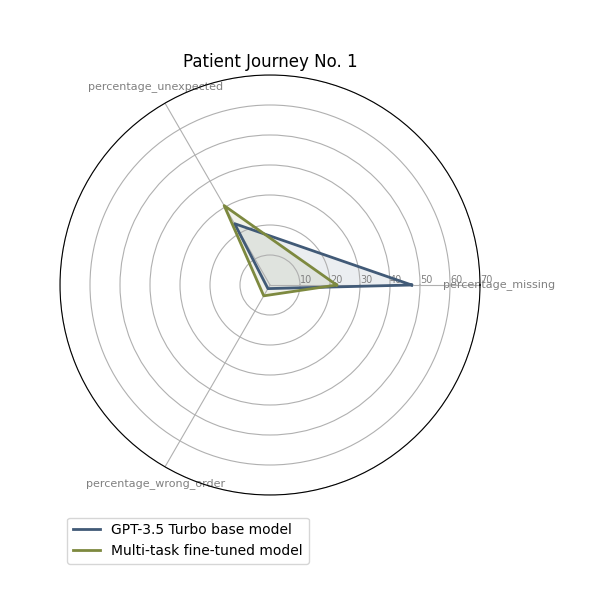
\includegraphics[width=0.3\textwidth]{bachelor_thesis/images/activites_pj1.png}}
  \subfigure[Patient Journey Nr. 2]{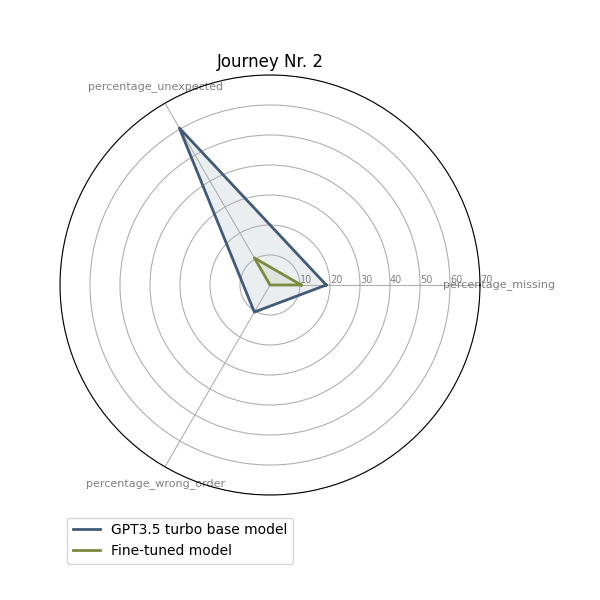
\includegraphics[width=0.3\textwidth]{bachelor_thesis/images/activites_pj2.png}}
  \subfigure[Patient Journey Nr. 3]{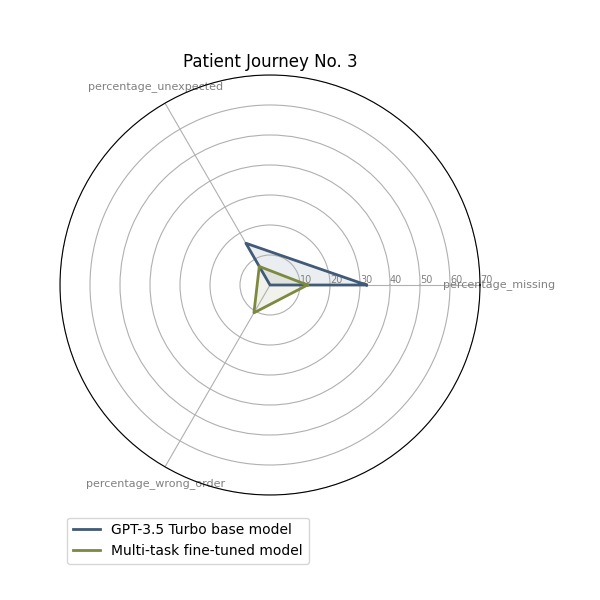
\includegraphics[width=0.3\textwidth]{bachelor_thesis/images/activites_pj3.png}}
  \subfigure[Patient Journey Nr. 4]{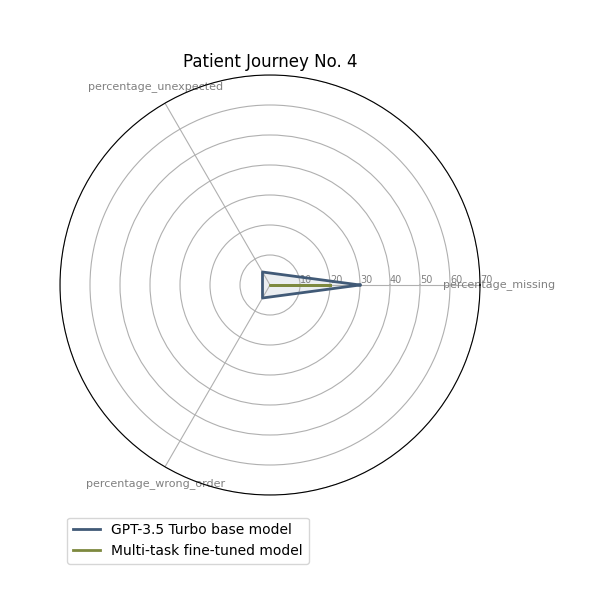
\includegraphics[width=0.3\textwidth]{bachelor_thesis/images/activites_pj4.png}}
  \subfigure[Patient Journey Nr. 5]{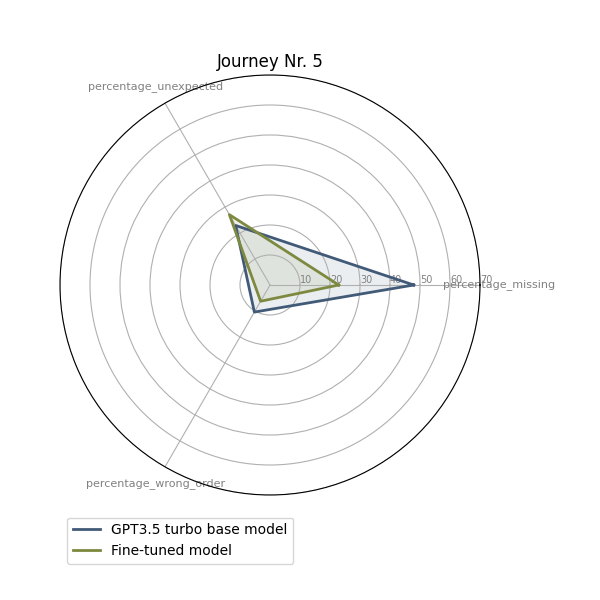
\includegraphics[width=0.3\textwidth]{bachelor_thesis/images/activites_pj5.png}}
  \caption{Radar Plots comparing the extraction results of GPT-3.5 Turbo and the Multi-Task Fine-Tuned model for Patient Journey 1-5~\ref{apx:pjs} for the task \quotes{Activity Labelling}}
  \label{fig:eval_activities_rad}
\end{figure}
Figure~\ref{fig:eval_activities_bar} illustrates the performance of both models across all patient journeys in a bar plot. Each bar represents the error rate in one of the metrics and the bars of the same metric for, each Patient Journey of base- and fine-tuned model respectively, overlap each other. A smaller amplitude is desirable. Although the fine-tuned model performed slightly worse in some metrics, its overall supremacy is evident. Especially with Patient Journey~1,2 and 4 the difference is clearly notable.  We make the following observations:
\begin{enumerate}
    \item \emph{Wrong Order} is the error type with the least occurrences across both models. On an average, there are more \emph{Missing Activity} errors than \emph{Unexpected Activity} errors. This indicates, that both model tend to rather not include relevant event than include irrelevant or imaginary events.
    \item The quality of the results is as diverse as the Patient Journeys.
    \item Patient Journey Nr.~5, which we assess to be the most challenging, has the highest overall error rate. This hints to a correlation between lacklustre structure in the Patient Journeys and worse quality of the event log.
    \item The multi-task fine-tuned model overall outperforms the base-model, though not consistently
\end{enumerate}

\begin{figure}
    \centering
    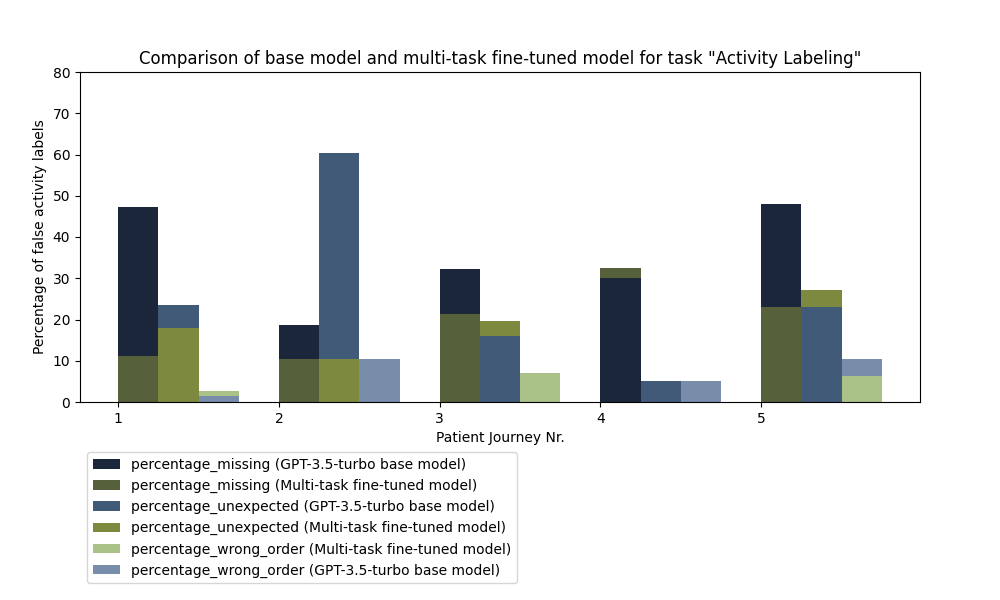
\includegraphics[width=\textwidth]{bachelor_thesis/images/activities_all.png}
    \caption{Bar Plot comparing the extraction results of GPT-3.5 Turbo and the Multi-Task Fine-Tuned model across all Patient Journeys~\ref{apx:pjs} for the task \quotes{Activity Labelling}} 
    \label{fig:eval_activities_bar}
\end{figure}

\paragraph{Event Type Classification} \autoref{fig:eval_event_types} shows the performance of both models across all patient journeys in a bar plot. Each bar represents the percentage of incorrectly classified event types.It is clear, that GPT-3.5 performs better on nearly every Patient Journey. This can have various reasons, like an under-representation of certain event types in the training data. We discuss the mater in \autoref{sec:discussion}. The gap between the two models is rather small, to a point where it can be almost considered negligible. Fine-tuning the model definitely did not increase the quality of the extraction results in this task. However, they are almost as good as the base models while not receiving examples in few-shot prompts with every request to the API. We discuss the matter of token consumption in \autoref{sec:eval_other}.
\begin{figure}
    \centering
    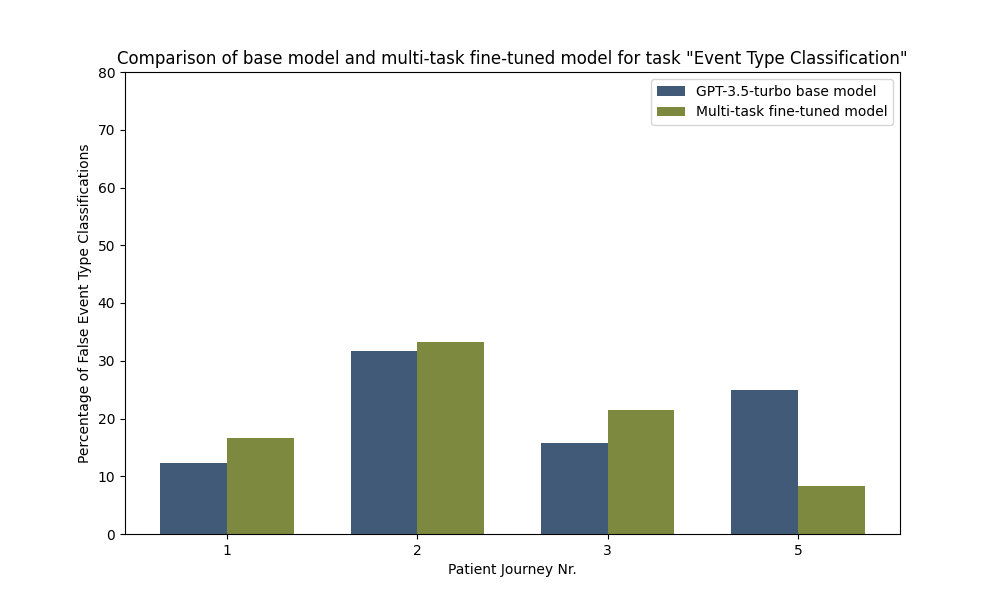
\includegraphics[width=\textwidth]{bachelor_thesis/images/event_types_all.png}
    \caption{Bar Plot comparing the extraction results of GPT-3.5 Turbo and the Multi-Task Fine-Tuned model across all Patient Journeys~\ref{apx:pjs} for the task \quotes{Event Type Classification}}
    \label{fig:eval_event_types}
\end{figure}

\paragraph{Timestamp Extraction}
The final task we trained the multi-task fine-tuned model for is extracting timestamps. \autoref{fig:eval_time} presents the ratio of incorrectly classified time stamps for both GPT-3.5 Turbo and the fine-tuned model. A smaller amplitude is desirable. We make the following observations:
\begin{enumerate}
    \item The error rate is considerably in this metric is higher than any other. This reflects our initial assessment, that the extraction of timestamps is the most difficult task out of the ones we evaluate in this thesis.
    \item the multi-task fine-tuned model achieved a better quality in almost every scenario. Especially the simpler Patient Journeys 2 and 4 were processed noticeably better. This indicates, that even the fine-tuned model struggles with the less well-structured description of time specifications and events with strong temporal relations.
\end{enumerate}
\begin{figure}
    \centering
    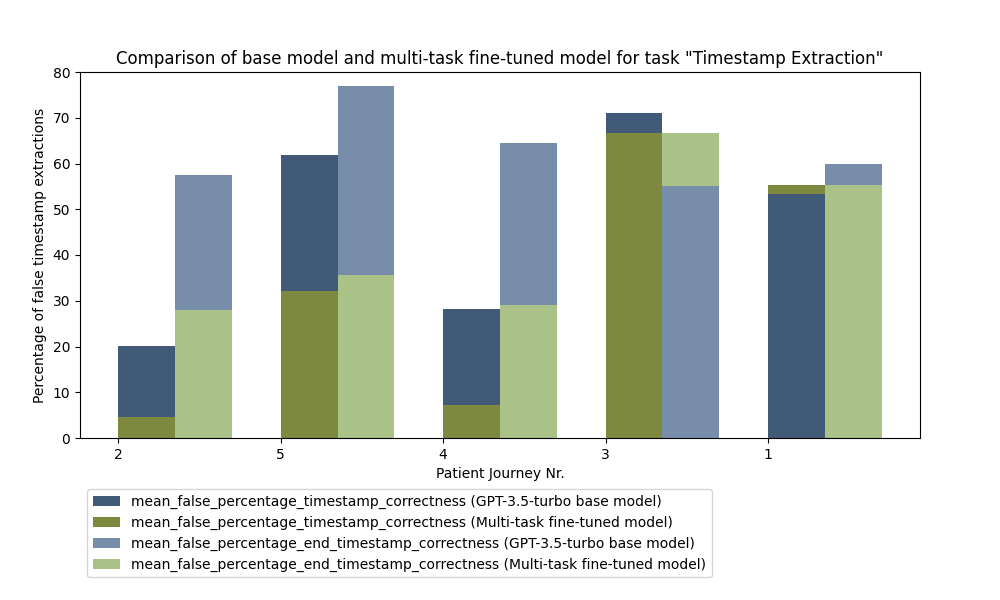
\includegraphics[width=\textwidth]{bachelor_thesis/images/timestamp_all.png}
    \caption{Bar Plot comparing the extraction results of GPT-3.5 Turbo and the Multi-Task Fine-Tuned model across all Patient Journeys~\autoref{apx:pjs} for the task \quotes{Timestamp Extraction}}
    \label{fig:eval_time}
\end{figure}


\subsubsection{Single-Task Fine-Tuned Model}\label{sec:eval_single}
The plots in \autoref{fig:eval_activities_single_rad} show comparisons of base model and single-task fine-tuned model in all three metrics for each Patient Journey individually. The axes each display the error rate in the extraction results the models achieved. A smaller amplitude is desirable.\\
\begin{figure}
  \centering
  \subfigure[Patient Journey Nr. 1]{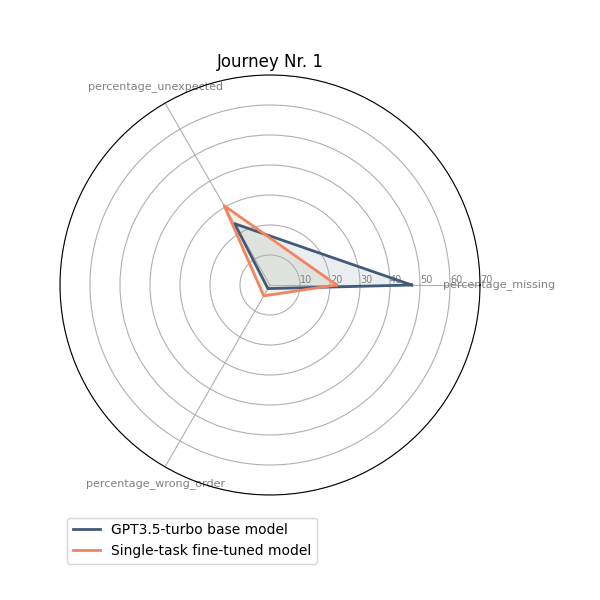
\includegraphics[width=0.3\textwidth]{bachelor_thesis/images/activites_pj1-single.png}}
  \subfigure[Patient Journey Nr. 2]{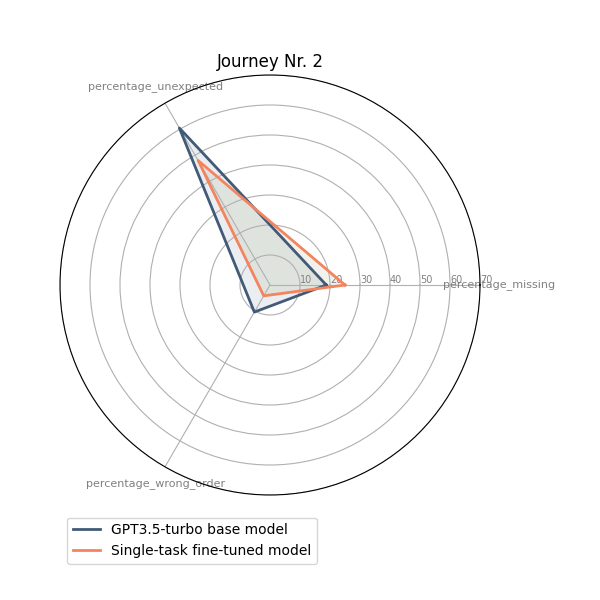
\includegraphics[width=0.3\textwidth]{bachelor_thesis/images/activites_pj2-single.png}}
  \subfigure[Patient Journey Nr. 3]{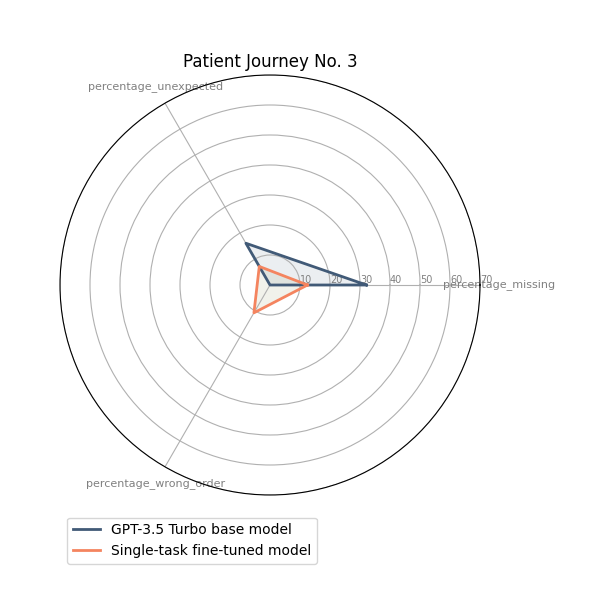
\includegraphics[width=0.3\textwidth]{bachelor_thesis/images/activites_pj3-single.png}}
  \subfigure[Patient Journey Nr. 4]{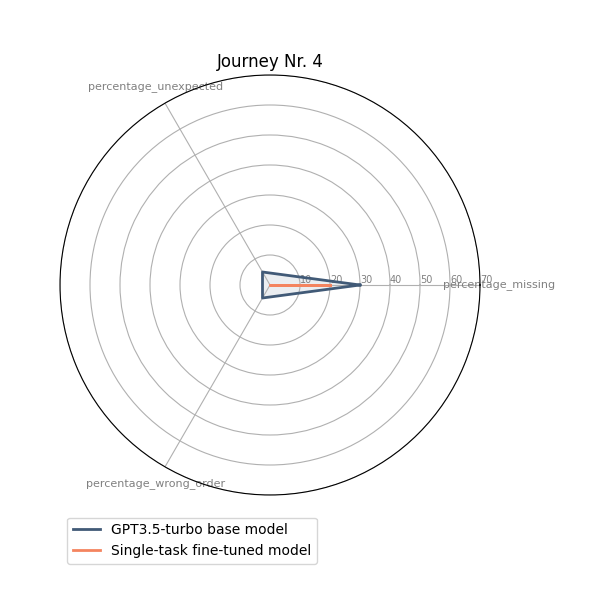
\includegraphics[width=0.3\textwidth]{bachelor_thesis/images/activites_pj4-single.png}}
  \subfigure[Patient Journey Nr. 5]{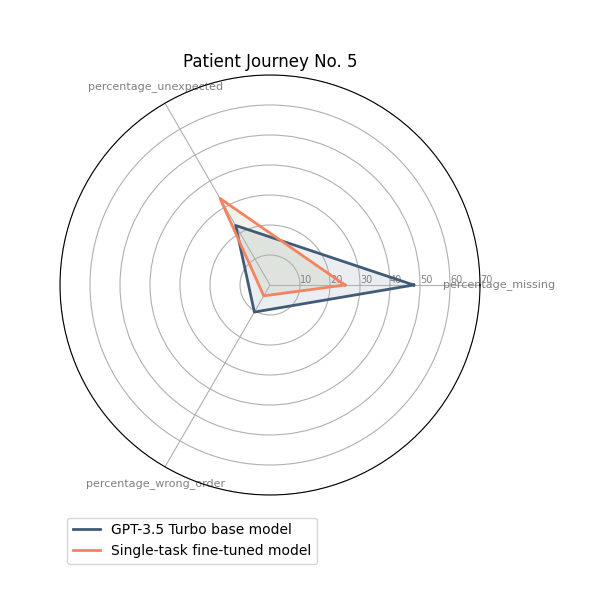
\includegraphics[width=0.3\textwidth]{bachelor_thesis/images/activites_pj5-single.png}}
  \caption{Radar Plots comparing the extraction results of GPT-3.5 Turbo and the Single-Task Fine-Tuned model for Patient Journey 1-5~\ref{apx:pjs} for the task \quotes{Activity Labelling}}
  \label{fig:eval_activities_single_rad}
\end{figure}
\autoref{fig:eval_activities_all_bar} illustrates the performance of both models across all patient journeys in a bar plot. Each bar represents the error rate in one of the metrics and the bars of the same metric for, each Patient Journey of base- and fine-tuned model respectively, overlap each other. A smaller amplitude is desirable. The fine-tuned model consistently scores better in the \emph{missing activity} metric, but only occasionally outperforms the base model in any other metric.
\begin{figure}
    \centering
    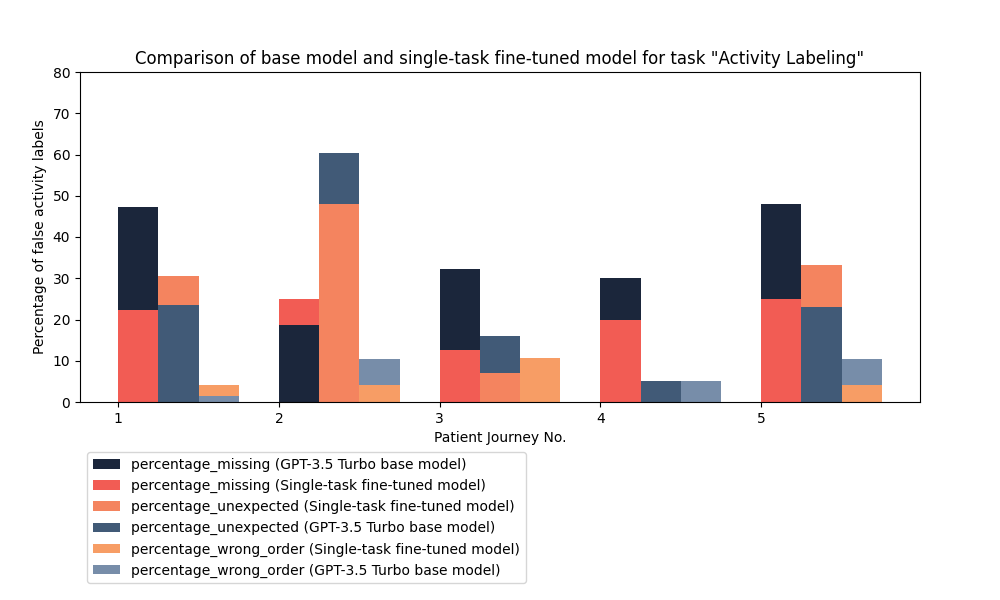
\includegraphics[width=\textwidth]{bachelor_thesis/images/activites_all-single.png}
    \caption{Bar Plot comparing the extraction results of GPT-3.5 Turbo and the Single-Task Fine-Tuned model across all Patient Journeys~\ref{apx:pjs} for the task \quotes{Activity Labelling}} 
    \label{fig:eval_activities_all_bar}
\end{figure}

\subsubsection{Comparison of Fine-Tuned Models}
Lastly, we compare the results of the two fine-tuned models in their mutual task \quotes{Activity Labelling}. As you can see in \autoref{fig:eval_activities_all_comparison_bar} the multi-task fine-tuned model performs better in 8 out of 15 measurements and the single-task fine-tuned model performs better in the other 7 measurements. All models performed notably good on Patient Journey 3 and 4, so these seem to be the easiest for an LLM to extract information from. The single-task fine-tuned model got the best scores for both of them. This indicates, that the specialisation on one task increases the performance in easier conditions while not increasing the performance under more difficult conditions. We further discuss this in~\autoref{sec:discussion}.

\begin{figure}
    \centering
    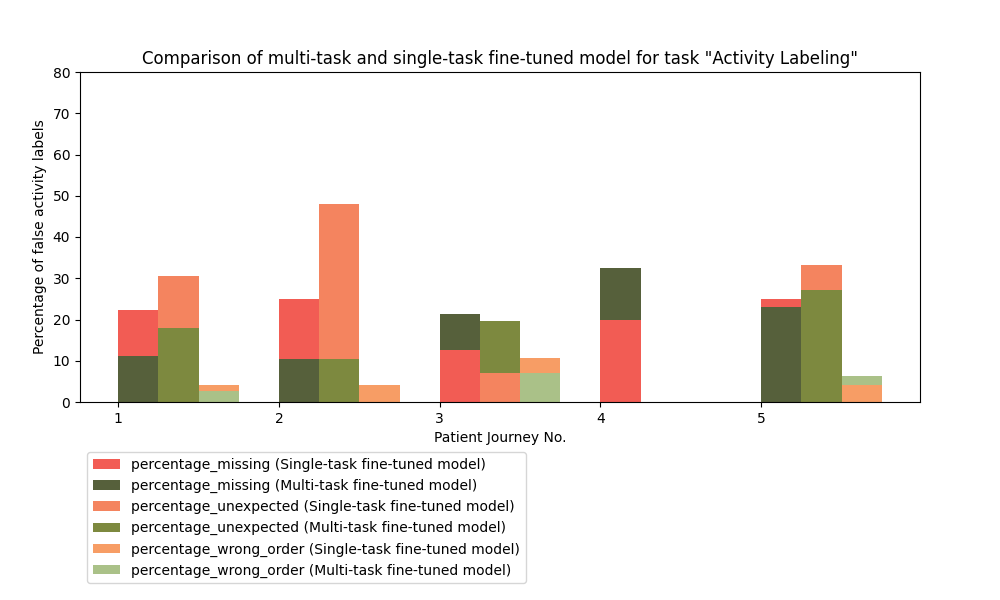
\includegraphics[width=\textwidth]{bachelor_thesis/images/activites_all-single_vs_multi.png}
    \caption{Bar Plot comparing the extraction results of multi-task and single-task fine-tuned model across all Patient Journeys~\ref{apx:pjs} for the task \quotes{Activity Labelling}} 
    \label{fig:eval_activities_all_comparison_bar}
\end{figure}

    \section{Discussion}\label{sec:discussion}
In this chapter, we will discuss the approaches and the results we achieved in hindsight.\\\\
Both approaches to fine-tuning improved GPT5.5 Turbo's performance. In some metrics, there are noticeably fewer improvements.\\
\begin{itemize}
    \item To our surprise, fine-tuning did not improve the model's capabilities in classifying event types for activities. This is the easiest of the four tasks we evaluated, and the base model performed reasonably well. The reason for that is likely a lack of diversity in the training data. In many Patient Journeys, events of type System Onset are more common than Treatment or Medication because patients can describe how they felt and experienced in more detail, compared to treatment and medication plans. Our training data reflects that.
    \item The single-task fine-tuned model performed worse or on par with the multi-task fine-tuned model in their mutual task. This is not necessarily an issue. The model learns from all the examples we provide during training and will what it learned in every response. Consequently, the examples intended to train the model for Event Type Classification can also improve its performance in Activity Labelling. Even though the single-task fine-tuned model received twice as many examples for the task \quotes{Activity Labelling} than the multi-task fine-tuned model, the overall number of examples was lower. The conclusion is that multi-task fine-tuning, in this case, is the superior approach. More training data could tip the scale, however.
\end{itemize}
The focus of \autoref{sec:fine} is selecting the correct training data and assembling data sets that the model can benefit from the most. We discussed various approaches and reasoned why one is better than the other. This relies on our experimentation, previous research, and claims made by OpenAI. Ultimately, all models we used are black-boxes, and there is no way to comprehend how exactly GPT-35.5 Turbo digested the data we provided.
	\section{Conclusion}\label{sec:conclusion}
This chapter completes the thesis. We will first summarize or work and our findings, discuss the limitations of the presented work and then outline the potential future work, that can make up for some of the limitations and extend the findings of our research.\\\\
Fine-tuning is an active research topic in the pursuit of increasing the performance of LLMs also in information extraction tasks. Extracting information from natural language text to create event logs poses some additional challenges, and Patient Journeys have proven to be inconsistent information sources.\\
We showed, that applying fine-tuning strategies to publicly available and affordable models can increase the quality of the extracted results, even with small amounts of training data. Especially noteworthy is the improvement in correctly determining and summarizing all relevant events in a specified context. We demonstrated that with Patient Journeys which describe Covid-19 courses of disease.\\
In combination with the successes in two of the other three evaluated tasks (extracting start and end timestamps), that both pose individual challenges, we conclude that fine-tuning, and SFT in particular, is indeed a valuable approach for improving the extraction of event logs from Patient Journeys.

\subsection{Limitations}\label{sec:limitations}
The approaches presented in \autoref{sec:fine} show some limitations. In the following paragraphs we disclose and discuss these limitations.\\\\
Attaining optimal results in extracting event logs from Patient Journeys with LLMs necessitates accounting for several critical factors. Foremost among these is the quality of input; substandard input leads to substandard output. This factor however can usually not be controlled.\\\\
Ensuring a well-formulated prompt is imperative, as prompt engineering should invariably precede fine-tuning in efforts to enhance quality.
In this research, prompts are deliberately excluded as a variable, with the most current iterations from TracEX being employed. While these prompts are not without flaws and likely possess potential for enhancement, the main objective of this study is to assess the efficacy of fine-tuning in extracting event logs from Patient Journeys. This evaluation is conducted through relative analyses; however, more definitive findings could be obtained if additional factors, such as the refinement of prompts, were also considered.\\\\
Fine-tuning is also intrinsically tied to the quantity of data available. Within the context of this bachelor’s thesis, the collection of training data is considerably constrained by time limitations. Absent these constraints, a greater quantity of data could be feasible, potentially leading to better outcomes.\\\\

\subsection{Future Work}\label{sec:future_work}
We want to point out three aspects that can be addressed in future work.\\
Future investigations should further probe the potential ceiling of fine-tuning in the context we discussed. Using unstructured text as a source for process information will likely become more important. Though this study demonstrates that fine-tuning can yield improvements, its ultimate limitations remain undetermined. Both of the presented approaches to fine-tuning use supervised fine-tuning (SFT) techniques. As outlined in \autoref{sec:fine-tuning-def} there are more techniques we considered, and many more we did not consider. Ultimately, we decided to use OpenAI's models and services for our approaches, which focus on SFT. Other techniques such as Retrieval Augmented Generation, Reinforcement Learning\cite{ovadia_fine-tuning_2024} or Iterative Refinement with Self-Feedback~\cite{madaan_self-refine_2023} might also yield great results. 
Using more training data and fine-tuning techniques could therefore be interesting.\\\\
Developing and applying even more discerning metrics could further improve the fine-tuning process required for extracting event logs from unstructured text. The metrics we introduced give us an indication for the performance of models on various tasks, but ultimately there is still a lot of information uncovered. Determining exactly what input characteristics restrict the model is therefore a fascinating research topic.\\\\
Furthermore, as publicly accessible models continue to evolve — exemplified by the recent release of GPT-4o — the scope of possibilities extends correspondingly. By 2026, innovations that are presently inconceivable are likely to become achievable. Therefore, future research should build on the more powerful LLMs we will surely see in the upcoming years.

    \csvstyle{Activities}{
tabular = |c|l|l|,
table head = \hline \textbf{Case ID} & \textbf{Activity} & \textbf{Event Type}\\\hline\hline,
late after line = \\\hline,
head to column names,
}
\csvstyle{SingleColumn}{
tabular = |l|,
table head = \hline \textbf{#1} \\\hline\hline,
late after line = \\\hline,
head to column names,
}
\section{Appendix}\label{sec:apx}
% \addcontentsline{toc}{section}{Appendix}
\addtocontents{toc}{\protect\setcounter{tocdepth}{-1}}
\subsection{Patient Journeys}\label{apx:pjs}
\subsubsection{Patient Journey 1}\label{apx:pj1}
I started experiencing symptoms of Covid-19 on July 15, 2021. As a 51-year-old teacher from Germany, I knew the importance of taking immediate action. I isolated myself at home and informed my family about the situation. Despite the financial difficulties we were facing, my main concern was the health and safety of my loved ones.\\
In the next few days, my symptoms worsened, and I decided to consult a doctor. I reached out to my family physician, who advised me to get tested for Covid-19. I made an appointment at a local testing center and underwent the necessary tests. The results confirmed my infection, and the doctor recommended home quarantine and symptomatic treatment.\\
During my isolation period, I focused on resting and following the doctor's advice. My loving wife took care of me and ensured that I had everything I needed. My children, understanding the seriousness of the situation, helped around the house and supported me emotionally.\\
As the weeks went by, I slowly recovered from the infection, thanks to the care and support of my family. I returned to work as a teacher, taking necessary precautions to protect both myself and my students.\\
In the following months, the Covid-19 situation began to improve, and vaccination campaigns were initiated. I made the decision to get vaccinated to further protect myself and those around me. I consulted with my doctor about the vaccine and its benefits for me as an individual. After careful consideration, I received my first dose of the vaccine in the month of September 2021.\\
Following the initial dose, I experienced mild side effects such as fatigue and soreness at the injection site. However, I remained optimistic and continued with my daily life while adhering to the safety guidelines.\\
In the weeks that followed, I received my second dose of the vaccine, completing the vaccination process. I felt a sense of relief and hope for the future, knowing that I had taken the necessary steps to protect myself and contribute to the collective effort of ending the pandemic.\\
Throughout this whole journey, I am grateful for the love and support I received from my family and the guidance of the healthcare professionals. Their care and expertise played a significant role in my recovery and ability to resume my work as a teacher.
\subsubsection{Patient Journey 2}\label{apx:pj2}
I started experiencing symptoms of Covid-19 on June 15, 2021. As a doctor, I immediately recognized the signs and knew I needed to take action. I self-isolated in a separate room of my house to protect my family and prevent any potential spread of the virus. The next day, I contacted my primary care physician and informed them about my symptoms.\\
Over the course of the next few days, my symptoms progressed, and I started experiencing high fever, cough, and fatigue. I diligently followed the guidelines provided by healthcare authorities, taking over-the-counter medication to manage my symptoms and staying hydrated. I continued to stay isolated at home, avoiding close contact with others.\\
Concerned about the severity of my symptoms, I reached out to a colleague who specialized in infectious diseases for a telemedicine consultation. They provided valuable advice on managing my symptoms and recommended regularly monitoring my oxygen levels using a pulse oximeter.\\
As the week progressed, my symptoms gradually improved. However, I remained cautious and continued to self-isolate to ensure the virus had fully run its course. After two weeks of isolation, I finally started feeling better and was able to resume my normal activities.\\
In terms of vaccination, after recovering from Covid-19, I decided to get vaccinated to provide additional protection against future infections. I received the first dose of the vaccine a few months later in September 2021, following the recommended schedule. I experienced mild side effects, including soreness at the injection site and fatigue, but they subsided within a few days.\\
I received the second dose of the vaccine in October 2021, completing the vaccination process. I followed up with my primary care physician to ensure I had developed a strong immune response to the virus. They reassured me that the vaccine would significantly reduce the likelihood of reinfection and the severity of any future infections.\\
Overall, my experience with Covid-19 highlighted the importance of following public health guidelines, seeking medical advice, and taking necessary precautions to protect both myself and my loved ones.
\subsubsection{Patient Journey 3}\label{apx:pj3}
As a 35-year-old doctor constantly on the go, juggling between patients and hospital rounds, I found myself infected with Covid-19 on August 15, 2022. It started with mild symptoms like fatigue and a slight cough, but quickly progressed to include body aches and a high fever. Concerned about the potential impact on my patients, I immediately isolated myself at home.\\
Over the next few days, my symptoms worsened, and I experienced difficulty breathing. Knowing the seriousness of the situation, I reached out to a fellow doctor for a virtual consultation. They advised me to monitor my oxygen levels regularly and prescribed medications to alleviate my symptoms. With their guidance, I managed to stabilize my condition and avoid hospitalization.\\
As the days passed, I realized the toll the virus was taking on my body. My energy levels were depleted, making it challenging for me to carry out my daily duties. Thankfully, my colleagues stepped in and offered to cover my hospital rounds, allowing me time to rest and recover.\\
In the following weeks, I focused on self-care, ensuring I followed a healthy diet, stayed hydrated, and got enough rest. I also relied on virtual support groups to connect with others who had experienced Covid-19, providing a sense of camaraderie during these difficult times.\\
With the recovery and discovery of vaccines, I made the decision to get vaccinated as soon as it became available to me. I received both doses of the vaccine within the recommended timeframe, which provided me with a sense of relief and protection against future infections.\\
Throughout this entire experience, I couldn't help but reflect on my single status. Being isolated during my illness made me long for companionship even more. As I approached my late thirties, I wondered if I would ever find love amidst my hectic schedule. However, I remained hopeful and determined to prioritize my health and well-being while keeping an open heart to whatever the future might hold.\\
In summary, my Covid-19 infection led me to take immediate action by isolating myself and seeking medical advice. I relied on virtual consultations, support groups, and the support of my colleagues to navigate through the challenging period of illness. Eventually, I seized the opportunity to get vaccinated, completing the recommended doses. The experience reinforced the importance of self-care and strengthened my resolve to find love despite the demands of my career.
\subsubsection{Patient Journey 4}\label{apx:pj4}
I had my first interaction with covid in early 2021. It all started with everyone getting back to school after the long break over the summer of 2020.\\
Because we were wearing masks all the time the immune system was really down. Idk how to say it, but every little cold hit harder than before. And that's why I didn't think much about it when I started coughing.But then it progressed to also fever but i never had typical problems like shortness of breath or all in all really heavy symptoms.I still went to school though as I had to prepare for my graduation, so I didn't test myself so i dont really know, if i really had it back then.However in the last weeks we had to test us every second day of school and some day in April i had a positiv test, so I had to go in quarantine and to get a negative pcr test like one week later at the local doctors'.\\
In this time I had no symptoms at all lol. I guess it was like october in 2021 when I finally got the first dose of vaccine against covid. The second was six or seven weeks later and someday in the first half of 22 i got the third round. I never understood antivaccers, but thats not my beer anyway...\\
I'm just happy that me and all people around me hadn't hard times with corona.
\subsubsection{Patient Journey 5}\label{apx:pj5} (Shortened from~\cite{malta_my_2020})\\
I'm a global health researcher working to address health and gender inequalities in the Global South. During my work in areas where Malaria or Dengue Fever are endemic, I always took extra precautions to avoid getting infected. I never anticipated that while living in a large, urban city from Canada I would be at higher risk… Until the COVID-19 pandemic.
During lockdown, like most working mothers, I became the major responsible for childcare and housework. To finish all my research related activities, I frequently worked until late at night. During the day I was juggling work, home and homeschooling… In mid May I started feeling weak and had more trouble breathing. As someone with an immunodeficiency disorder, I didn't pay too much attention. I though it was due to sleep deprivation and excessive working hours… But it was COVID-19. The symptoms worsened quickly and in a few days I was not able to get out of bed. Now I was under lockdown, unable to work or look after my kids, with stress piling up.\\\\
My physician considered the symptoms mild, recommending isolation and rest at home… I laughed: How does someone isolate and rest with three little kids at home and so much work to do? I was bedridden for three weeks, with difficulty breathing, headache, conjunctivitis, sore throat, aches and pain. I completely lost my appetite. During two months I could not taste or smell anything, hot or cold, sweet, salty, spice, nothing at all. My fatigue was debilitating. More than four months later, my symptoms have not gone away. My heart still races a few times a day - even while I am sitting at the computer and writing this piece. It is hard to concentrate for long periods. Imagine a scientist that cannot concentrate properly… That's me. What about the stress? It keeps piling up, with no light on the horizon.\\
I'm what has been identified as a ‘long-hauler’, those individuals who survived a COVID-19 infection but are enduring long-term symptoms. Fatigue is one of the most common symptom, while many report racing heartbeat, enduring achy joints and shortness of breath.\\\\
Like many long-haulers, my goal is to resume previous normal and productive life. However, I still experience a plethora of long-term symptoms, including extreme fatigue and brain fog. Many long-haulers fear unemployment, as they face incapacitating symptoms and/or lower productivity. The burden of having a possible long-term condition is very stressful. But when allied with the prospects of unemployment, and for many, loss of health insurance, it can be unbearable. I'm grateful for being alive, still employed and living in a country offering universal, publicly funded healthcare. Many don't have the same privilege.
\newpage
\subsection{Ground Truths}\label{apx:ground_truths}
\begin{table}[h]
    \tiny
    \captionsetup{justification=raggedright,singlelinecheck=false}
    \caption{Ground truth for Patient Journey 1~\ref{apx:pj1}}
    \csvreader[Activities]{bachelor_thesis/data/journey_comparison_1_ground_truth.csv}{event_type=\eventtype}{%
        1 & \activity & \eventtype
    }
    \label{tab:pj1-gt}
\end{table}
\begin{table}[h]
    \tiny
    \captionsetup{justification=raggedright,singlelinecheck=false}
    \caption{Ground truth for Patient Journey 2~\ref{apx:pj2}}
    \csvreader[Activities]{bachelor_thesis/data/journey_comparison_2_ground_truth.csv}{event_type=\eventtype}{%
        2 & \activity & \eventtype
    }
    \label{tab:pj2-gt}
\end{table}
\begin{table}[h]
    \tiny
    \captionsetup{justification=raggedright,singlelinecheck=false}
    \caption{Ground truth for Patient Journey 3~\ref{apx:pj3}}
    \csvreader[Activities]{bachelor_thesis/data/journey_comparison_3_ground_truth.csv}{event_type=\eventtype}{%
        3 & \activity & \eventtype
    }
    \label{tab:pj3-gt}
\end{table}
\begin{table}[h]
    \tiny
    \captionsetup{justification=raggedright,singlelinecheck=false}
    \caption{Ground truth for Patient Journey 4~\ref{apx:pj4}}
    \csvreader[Activities]{bachelor_thesis/data/journey_comparison_4_ground_truth.csv}{event_type=\eventtype}{%
        4 & \activity & \eventtype
    }
    \label{tab:pj4-gt}
\end{table}
\begin{table}[h]
    \tiny
    \captionsetup{justification=raggedright,singlelinecheck=false}
    \caption{Ground truth for Patient Journey 5~\ref{apx:pj5}}
    \csvreader[Activities]{bachelor_thesis/data/journey_comparison_5_ground_truth.csv}{event_type=\eventtype}{%
        5 & \activity & \eventtype
    }
    \label{tab:pj5-gt}
\end{table}
\addtocontents{toc}{\protect\setcounter{tocdepth}{2}}
    \listoffigures
    \addcontentsline{toc}{section}{List of Figures}
    \lstlistoflistings
    \addcontentsline{toc}{section}{List of Listings}
    \listoftables
    \addcontentsline{toc}{section}{List of Tables}

	% bibliography
	\cleardoublepage
	\renewcommand{\refname}{References}
	\bibliographystyle{plain}
	\bibliography{bibliography/references}

\end{document}